\hfuzz=5pt % Allow up to 5pt of overfull without warning
\hbadness=10000 % Suppress underfull warnings

\section{Chapter 4 - Pauline Epistles to All Nations}\label{sec:chapter-4---pauline-epistles-to-all-nations}

πορευθέντες οὖν μαθητεύσατε πάντα τὰ ἔθνη ``Go, therefore, and make disciples of all nations.''

The key point missed by most scholars is that \textit{panta ta ethnē} does not refer to ``all nations'' universally, but rather to the nations of the Greek world.
The Septuagint consistently uses \textit{ethnē} to describe the nations under God's rule---those invited into covenant---not every nation globally.
In Hellenistic inscriptions, the phrase ``all the nations'' (\textit{panta ta ethnē}) is repeatedly used to describe the \textit{oikoumene}, the civilized world subject to the emperor.
It was imperial language, not global anthropology.
Thus, Matthew’s Great Commission is not an open-ended call to the Americas or India, but to the Greek-speaking nations of the empire.

Καὶ εὐλογηθήσονται ἐν τῷ σπέρματί σου πάντα τὰ ἔθνη τῆς γῆς ``And in your seed, all the nations of the earth shall be blessed.''
This is a key passage used in early Christianity (Galatians 3:8) to show that all the nations were meant to be part of God's covenant, not just outsiders.

Βασιλεῖς τῆς γῆς καὶ πάντες λαοὶ, ἄρχοντες καὶ πάντες κριταὶ γῆς\ldots{} ὑψώσεως κεράτων λαοῦ αὐτοῦ, ὕμνος πᾶσι τοῖς ὁσίοις αὐτοῦ, τοῖς υἱοῖς Ἰσραὴλ, λαῷ ἐγγίζοντι αὐτῷ.
``Kings of the earth and all peoples, rulers and all judges of the earth\ldots{} a hymn for all His saints, the sons of Israel, a people near to Him.''
The ``kings of the earth and all peoples'' are brought into God's rule, but the focus remains on God's people.

All nations referred to God's people, not necessarily only Greek ethnicity, but all nations who proclaimed the rule of God.
So that would also include Jews and any other nation integrated into the imperial covenant.

\paragraph{1.
The early dating of the gospels can make the letters of Paul more plausible as it seems Paul already has the knowledge of at least one of the gospels and the acts.}\label{par:the-early-dating-of-the-gospels-can-make-the-letters-of-paul-more-plausible-as-it-seems-paul-already-has-the-knowledge-of-at-least-one-of-the-gospels-and-the-acts.}

Many scholars dispute the existence of Paul based on the striking contradiction in mainstream scholarship that authors of Pauline epistles seem to have the knowledge of the gospels and the acts, and yet the gospels and the acts are unanimously dated to be written after the Pauline epistles.
In here the existence of Paul can once more be reconsidered if we acknowledge the early dating of the gospels and the gospel of John in being written by an eyewitness of Jesus's life.

\paragraph{2.
What is quite striking is that Paul and others write to so many different churches over the short period of time.}\label{par:what-is-quite-striking-is-that-paul-and-others-write-to-so-many-different-churches-over-the-short-period-of-time.}

There is a major challenge for the traditional timeline of the apostles establishing so many churches in such a short period of time.
These churches would have to all be established, grow, keep up to date with the fastly shifting theology, and then do nearly nothing for the next 100 years.
These churches immediately showed up in every single major city in the former Greek empire, and no churches showed up anywhere else.
All of the correspondence and scripture was written in Greek, and no other languages.
It is important to point out that Greek was absolutely not the lingua franca in any part of the Roman empire that was not recently part of the Greek empire.
The lingua franca of the Roman empire was Latin, and that was the only language that was used in the administration and the primary language used by the authors.
If the apostles were to establish churches everywhere in the Roman empire, and not just in the former Greek empire, then we would have had the epistles to the extremely prominent cities of Mediolanum, Lutetia, Aquilea, Lugdunum, Memphis, and Londinium.
The truth is that no matter how we model the growth of the early church, it is not possible to explain the the patterns we observe.
And then for the next 100 years do not add any new churches.

Even more striking is the total absence of Aramaic or Hebrew letters.
If the apostles’ mission were Jewish in nature, at least some correspondence would survive in the languages of Judea.
Instead, all the letters are in Greek, to Greek assemblies, proving that the movement was imperial and Hellenistic at its core.

\paragraph{2a.
Paul’s letters as state correspondence.}\label{par:pauls-letters-as-state-correspondence.}

The epistles resemble circular letters of the Hellenistic and Roman administrations.
They are addressed to \textit{ekklesiai}, the same word used for political assemblies of citizens in Greek cities.
Paul is not writing to small house cults, but to recognized civic assemblies under a higher king.
This gives the Pauline corpus the character of imperial decrees rather than private exhortations.

There were essentially no prominent cities in the former Greek empire that were not mentioned in the Acts and the epistles:

% --- tables unchanged here ---

It is important to actually visualize the locations mentioned in the Acts and the epistles to see the striking pattern of the locations mentioned in the Acts and the epistles being the same as the most significant Greek speaking cities.

\begin{figure}[ht]
    \centering
    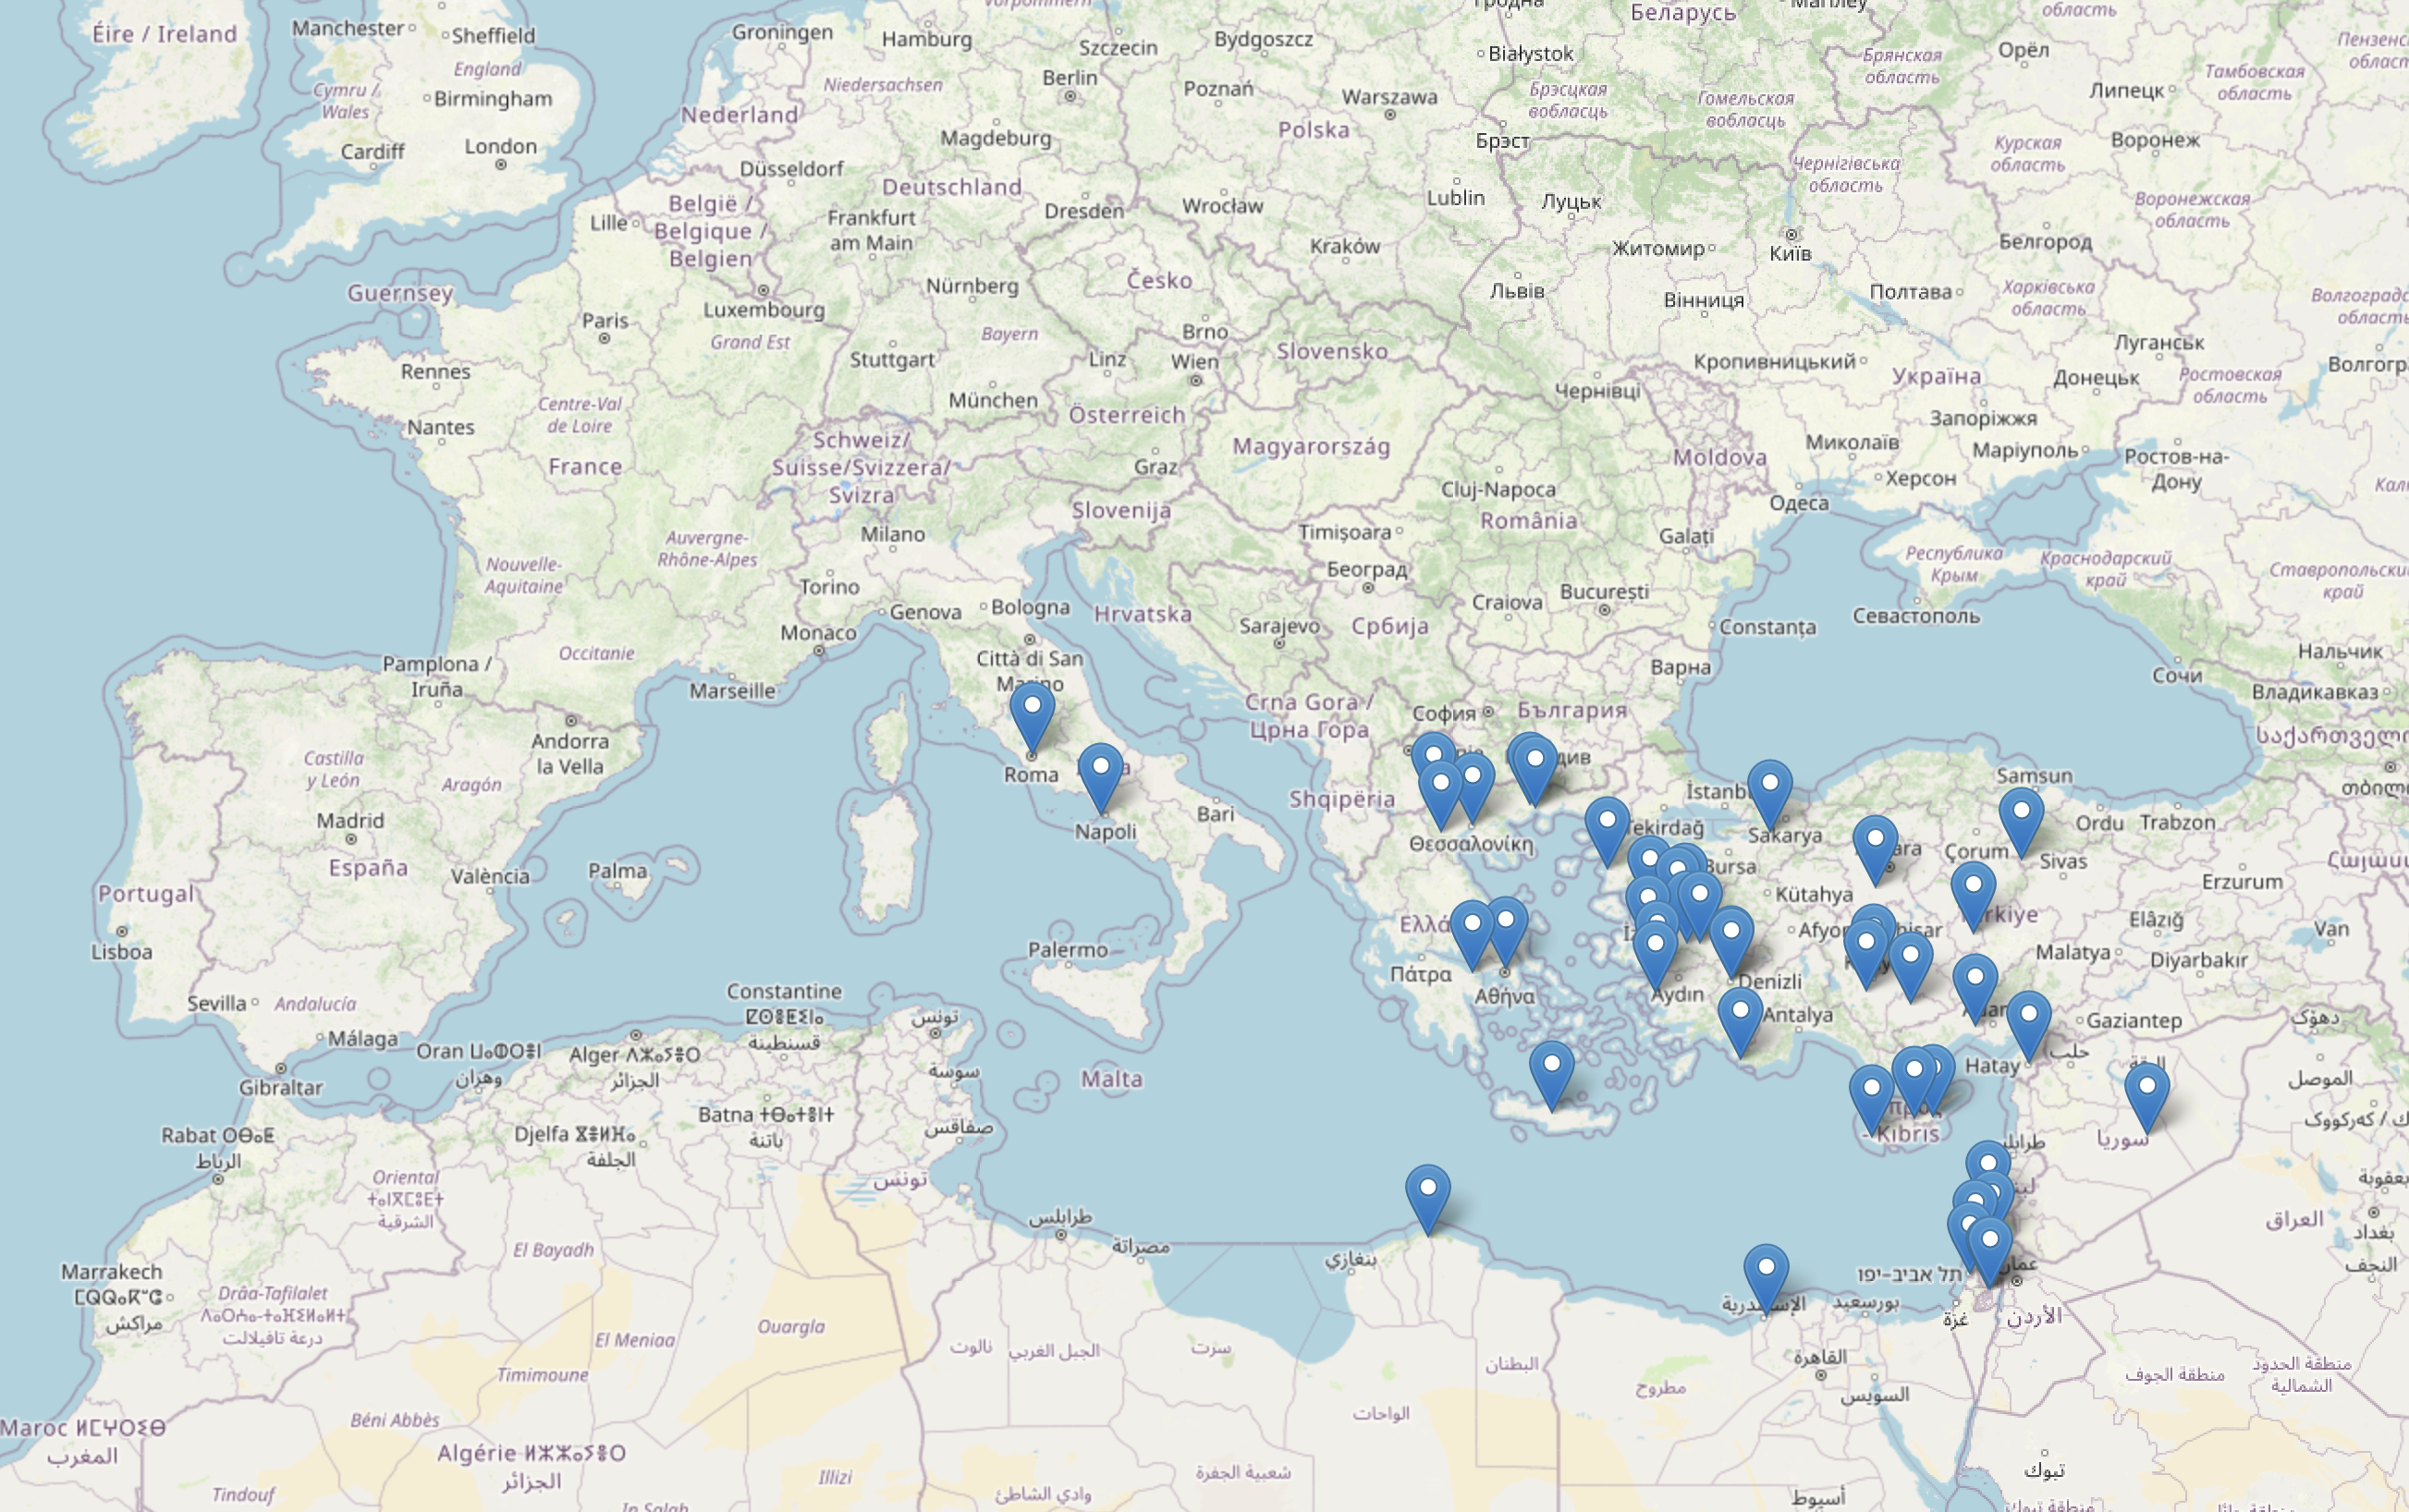
\includegraphics[width=\textwidth, keepaspectratio]{assets/locations_map}
    \caption{Map of all the locations mentioned in the Acts and the epistles.}
    \label{fig:figure}
\end{figure}

For those geographically inclined you can spot the near perfect correlation with the borders of Eastern Roman Empire.
Of note is the trip to Rome, which was substantially different in nature to the other trips.
\href{https://en.wikipedia.org/wiki/Byzantine_Empire_under_the_Theodosian_dynasty\#/media/File:4KTHEODOSIAN.png}{Rome Map}

\paragraph{3.
The striking statistics of the cities mentioned in the Acts and the epistles are that they are all in the former Greek empire, and not one mention of a city in the Roman empire that was not part of the former Greek empire.}\label{par:the-striking-statistics-of-the-cities-mentioned-in-the-acts-and-the-epistles-are-that-they-are-all-in-the-former-greek-empire-and-not-one-mention-of-a-city-in-the-roman-empire-that-was-not-part-of-the-former-greek-empire.}

This fact makes any theory that deems Christianity as a religious and not a political movement immediately highly implausible.

\paragraph{4.
Finally we consider the apparent minimal resistance to the acceptance of the new religion.}\label{par:finally-we-consider-the-apparent-minimal-resistance-to-the-acceptance-of-the-new-religion.}

The new religion was accepted by the masses in the former Greek empire, and not a single mention of any resistance to the new religion from the Greeks themselves.
The only real opposition comes from the Temple authorities in Jerusalem.
This is consistent with Christianity being a continuation of Greek imperial philosophy, which the Hellenized population already accepted.

\paragraph{5.
We should also consider that even though the religion was so successful at converting the masses, it still had all the conspiratorial parts to it.}\label{par:we-should-also-consider-that-even-though-the-religion-was-so-successful-at-converting-the-masses-it-still-had-all-the-conspiratorial-parts-to-it.}

Early Christians used secret symbols to identify each other, they frequently met in secret, often at night in the catacombs.
This is not unlike the initiation practices of other imperial soldier cults such as Mithras.
The Pauline language of ``soldiers of Christ'' fits this conspiratorial military model.

\paragraph{6.
Consider why the religion was seemingly much more prosecuted than any other religion in the Roman empire.}\label{par:consider-why-the-religion-was-seemingly-much-more-prosecuted-than-any-other-religion-in-the-roman-empire.}

The Roman empire was very tolerant of other religions, and the only time they would prosecute a religion was if it was a threat to the empire.
Christians were persecuted not for worshipping a strange god, but for refusing the Roman emperor cult while insisting that only their Christ was king.
This was a political treason, not theological quibbling.

\paragraph{7.
The phrase ``soldiers of Christ'' is not used explicitly in the Gospels, but it appears prominently in the Pauline Epistles.}\label{par:the-phrase-soldiers-of-christ-is-not-used-explicitly-in-the-gospels-but-it-appears-prominently-in-the-pauline-epistles-particularly-in-the-context-of-the-christian-life-being-compared-to-a-military-struggle-or-a-spiritual-battle.}

The metaphor emphasizes loyalty, discipline, and readiness for conflict under a divine king.
It reflects the military cultic environment of the empire, not a rural Jewish sect.

\paragraph{8.
Paul barely mentions the life of Jesus, and almost never quotes him.}\label{par:paul-barely-mentions-the-life-of-jesus-and-almost-never-quotes-him.}

It is frequently claimed that Paul's religion is not the religion of Jesus, but the religion about Jesus.
There is a shocking lack of references to any of the teachings of Jesus, the Jewish law, and any of the events surrounding Jesus's life and death.
So we may go one step further.
It is a religion focusing on restoring the kingdom of God by resurrecting the office of the Christos, the rightful king of the kingdom of God.
And so to Paul and all the early Christians, it was all about resurrecting a Christ, not teachings of the particular Jesus Christ.
The idea that God will once again send a king that will restore the Greek empire, the kingdom of God, headed by Christos, the rightful earthly king of the kingdom of God.

\paragraph{9.
Using this conspiratorial language clearly worked.}\label{par:using-this-conspiratorial-language-clearly-worked}

Rome did not even realize the new religion's goal was to restore the Eastern Empire until it actually happened.

\paragraph{10.
Alexandria was the capital of the Greek Empire and the center of the Hellenistic world and yet there are no missions or letters to Alexandria.}\label{par:alexandria-was-the-capital-of-the-greek-empire-and-the-center-of-the-hellenistic-world-and-yet-there-are-no-missions-or-letters-to-alexandria.}

The absence of Alexandria in the New Testament is striking, especially considering its significance.
Alexandria was erased from the text, as it was the origin city of Apollos, as well as some of the other companions of Paul such as Mark, Demas, and Luke.
The omission is best explained as deliberate suppression, precisely because Alexandria was already the center of the movement.
Just as the Old Testament largely omits the Ptolemaic empire despite its centrality, so the New Testament minimizes Alexandria while still presuming its leadership.

\subsection{Acts of the Apostles}\label{subsec:acts-of-the-apostles}

Is called the Acts of the Apostles, not acts of the disciples.
Apostles doing imperial work of letting all nations of the empire know the will of the God king.

\paragraph{10.
Acts opens with a royal enthronement}\label{par:acts-opens-with-a-royal-enthronement}

Acts 1:6 --- ``Lord, will you at this time restore the kingdom to Israel?'' This is not a spiritual question.
It implies Jesus had a claim to political kingship.
Your theory: Jesus was understood as the rightful monarch of a revived kingdom---a successor to the Herodian or Hasmonean thrones under Greek imperial ideals.

\paragraph{10.
Jesus is taken up like an emperor}\label{par:jesus-is-taken-up-like-an-emperor}

Acts 1:9--11 --- The Ascension mimics apotheosis scenes (e.g., Alexander, Roman emperors).
It frames Jesus in imperial terms, being enthroned in heaven---like a divine emperor.
This matches your view that Christianity was about loyalty to the ``Christ Emperor.''

\paragraph{10.
The Pentecost scene mimics an imperial inauguration}\label{par:the-pentecost-scene-mimics-an-imperial-inauguration}

Acts 2 --- Multilingual miracle and mass conversion reflects the imperial ideal of uniting nations under one divine king.
The language of ``tongues'' is political: the emperor's message is for all nations.

\paragraph{10.
Acts 5: The trial of the apostles}\label{par:acts-5-the-trial-of-the-apostles}

Gamaliel references past revolutionary figures---Theudas and Judas the Galilean.
This acknowledges that messianic revolts were political, and that Jesus' movement was seen in similar terms.

\paragraph{10.
Stephen's speech in Acts 7 is anti-Temple}\label{par:stephens-speech-in-acts-7-is-anti-temple}

Stephen attacks the Temple and Mosaic tradition, echoing Philo and Stoic-influenced criticisms of Jewish legalism.
This supports the view that early Christianity rejected the Mosaic religion and aligned more with philosophical monotheism.

\paragraph{10.
Paul as imperial envoy}\label{par:paul-as-imperial-envoy}

Paul appeals to Caesar, travels through Greek cities, and preaches to Hellenized elites.
His speeches (e.g., Acts 17 in Athens) are clearly political-philosophical, not sectarian Jewish.
Acts frames Paul as a philosopher-diplomat for the Christ-emperor.

\paragraph{11.
Acts ends without resolution}\label{par:acts-ends-without-resolution}

The book ends in Rome, with Paul freely preaching ``the kingdom of God.''
It lacks a narrative climax because its real message is that the empire is now Christian.
It presumes a pre-existing audience that sees Christianity as a political-theological force.

\subsubsection{James the Just}\label{par:james-the-just}

\paragraph{1.
James the Just also wrote an epistle to all nations.}\label{par:james-the-just-also-wrote-an-epistle-to-all-nations.}

He was the brother of Jesus, and the next in line to the throne.
Much like Jesus Christ the Soter, James also held a royal title, the Just.

James the Just also wrote an epistle to all nations, which is included in the New Testament.
James, like John, refers to the same understanding of Logos as Philo of Alexandria.
The writing style of James and John also bears a striking resemblance to the writing style of Philo of Alexandria.

In Greek, James 1:21 reads as:
``Διὸ ἀποθέμενοι πάσαν ἀκαθαρσίαν καὶ περισσείαν κακίας ἐν πραΰτητι δέξασθε τὸν ἐμφυτον λόγον, ὃς δύναται σῶσαι τὰς ψυχὰς ὑμῶν.''
Transliteration: ``Dio apothemenoi pasan akatharsian kai perisseian kakias en prautēti dexasthē ton emphuton logon, hos dynatai sōsai tas psychas hymōn.''
A literal translation: ``Therefore, putting away all filthiness and the overflow of wickedness, with meekness receive the implanted word, which is able to save your souls.''

It should go without saying that the advanced writing style of James and John is not something that would be expected from a simple fisherman or a son of a carpenter.
Rather, it confirms Alexandrian philosophical schooling at the very center of the Greek imperial world.

\subsubsection{The Epistles of John}\label{par:the-epistles-of-john}


\subsection{The Corpus of the New Testament}\label{subsec:the-corpus-of-the-new-testament}

What is actually in the New Testament, and how does it map onto the four imperial poles we have identified?
Below we make the mapping explicit \emph{and} anchor it with specific ancient evidence, especially for the epistles and early authorship claims.
Note well: in antiquity the attributions of the four canonical gospels to \textit{Matthew, Mark, Luke, John} are uniformly asserted by the Fathers.
No alternative apostolic names are recorded for them.

\paragraph{Patristic attestations (authorship in antiquity).}
Before the mid–third century the picture is consistent.
\textbf{Papias} (via Eusebius, \textit{Hist.\ Eccl.} 3.39) — Mark wrote as Peter’s interpreter.
Matthew compiled the \textit{logia}.
\textbf{Irenaeus} (\textit{Adv.\ Haer.} 3.1.1) — explicitly lists and defends the four: Matthew, Mark, Luke (Paul’s companion), John.
The \textbf{Muratorian Fragment} (late 2nd c.) names Luke and John as the third and fourth gospels and recognizes a Pauline corpus.
\textbf{Clement of Alexandria} and \textbf{Origen} repeat these attributions.
\textbf{Eusebius} later summarizes them as received.
For epistles: \textbf{1~Clement} (c.~96) cites 1~Corinthians.
\textbf{Ignatius} (c.~110) presupposes Pauline churches and diction.
\textbf{Polycarp} (c.~135) quotes or echoes multiple Pauline letters and 1~Peter.
\textbf{Irenaeus} uses 1–2~Peter, 1~John, and James as apostolic.
Discussion about Hebrews’ author and the lateness of 2~Peter appears later.
Crucially, there is no early counter–attribution of the \emph{four gospels} to other names.

\paragraph{Papyri and early circulation (snapshot).}
\textbf{P\textsuperscript{46}} (c.~200) preserves a Pauline collection (Rom, 1–2~Cor, Gal, Eph/Col, Phil, 1~Thess, Heb), showing the letters already circulated as a corpus.
\textbf{P\textsuperscript{66}} (c.~200) and \textbf{P\textsuperscript{75}} (early 3rd c.) are major early witnesses to John (and Luke/John).
\textbf{P\textsuperscript{9}} (3rd c.) preserves 1~John at Oxyrhynchus.
\textbf{P\textsuperscript{72}} (3rd/4th c.) contains 1–2~Peter and Jude.
\textbf{P\textsuperscript{13}} (3rd c.) Hebrews.
\textbf{P\textsuperscript{45}} (3rd c.) Gospels/Acts.
These confirm early circulation and natural clustering (Pauline set; Petrine/Jude; Johannine) that mirrors our four-pole architecture.
Egyptian findspots reflect preservation bias.
The \emph{composition} clustering still tracks the imperial map.

\paragraph{Johannine (Egypt / Ptolemies).}
\textbf{Gospel of John} is the Alexandrian gospel, written in the idiom of Logos theology.
In our framework it preserves the testimony of the Beloved Disciple (the woman whom Jesus loved) and originated in Egypt.
The \textbf{Epistles of John} (1–3~John) extend the same idiom (light/dark, truth/lie, the Word manifested).
They consolidate Egyptian \textit{ekklesiai} under the royal claim of Christ.
They insist on embodied loyalty (“what we have heard, seen, handled”) and police schism.
\emph{Early evidence:} Irenaeus quotes John and 1~John as apostolic.
P\textsuperscript{66} and P\textsuperscript{75} (John) and P\textsuperscript{9} (1~John) are among our earliest witnesses.
The Muratorian Fragment includes Johannine Catholic epistles.
\emph{We deliberately do not bundle Revelation here.}
It will be treated separately.

\paragraph{Matthean (Judea / Herodians).}
\textbf{Gospel of Matthew} is the Judean gospel: Jesus as true King of the Jews and new Moses, fulfilling and surpassing Torah.
Partner writings: \textbf{James} (by James the Just, the royal brother who led Jerusalem) and \textbf{Jude} (self-identified brother of James).
\emph{Early evidence:} Papias on Matthew.
Irenaeus and the Muratorian Fragment list Matthew.
Origen and Eusebius affirm Jacobean authorship.
Early Catholic lists include Jude.
James’ concise Greek moral style fits Alexandrian/Jerusalem schooling at the imperial center.

\paragraph{Lukan–Pauline (Aegean / Greeks).}
\textbf{Gospel of Luke} is the Aegean gospel: historiographic prologue (\textit{kratiste Theophile}), polished Greek.
It continues in \textbf{Acts}.
The corpus pairs with the \textbf{Pauline epistles} — letters to \textit{ekklesiai} in the Aegean and Asia Minor: \textit{Romans} (from Corinth), \textit{1–2~Corinthians}, \textit{Galatians} (interior Anatolia), \textit{Philippians} (Macedonia), \textit{1–2~Thessalonians} (Macedonia), \textit{Ephesians}/\textit{Colossians} (Asia), \textit{Philemon}.
\emph{Early evidence:} 1~Clement refers to Paul’s Corinthian correspondence.
Ignatius addresses Pauline cities and adopts Pauline diction.
Polycarp quotes Paul repeatedly.
The Muratorian Fragment enumerates a Pauline corpus.
P\textsuperscript{46} attests a bound collection.
Luke’s tie to Paul is ancient: Col 4:14; Phlm 24; 2~Tim 4:11; and the “we” sections in Acts.

\paragraph{Markan–Petrine (Seleucid East / Syria–Anatolia).}
\textbf{Gospel of Mark} is the Seleucid gospel, proclamation in rough Greek with Aramaic traces, suited to Antioch–Syria–Anatolia.
It preserves Peter’s preaching in written form.
The partner epistle is \textbf{1~Peter}, addressed explicitly to the Seleucid frontier provinces (“Pontus, Galatia, Cappadocia, Asia, Bithynia,” 1~Pet 1:1).
\emph{Early evidence:} Papias on Mark as Peter’s interpreter.
Irenaeus locates Mark after Peter and Paul.
1~Peter’s destination list maps our Seleucid frontier.
P\textsuperscript{72} later transmits 1–2~Peter with Jude in an eastern Catholic collection.

\paragraph{Epistolary map (evidence at a glance).}
\begin{center}
\begin{tabular}{@{}p{3.1cm}p{3.3cm}p{3.8cm}p{4.0cm}@{}}
\toprule
\textbf{Epistle} & \textbf{Addressees / Region} & \textbf{Earliest patristic attestation} & \textbf{Earliest papyrus witness} \\
\midrule
Romans & Rome (from Corinth) / Aegean network & 1~Clement; Ignatius; Polycarp & P\textsuperscript{46} \\
1–2 Corinthians & Corinth / Aegean & 1~Clement 47 cites 1~Cor; Polycarp & P\textsuperscript{46} \\
Galatians & Anatolian interior & Irenaeus; Polycarp echoes & P\textsuperscript{46} \\
Ephesians/Colossians & Asia (circular) & Ignatius (Eph); Irenaeus & P\textsuperscript{46} \\
Philippians & Macedonia & Polycarp (to Philippi) & P\textsuperscript{46} \\
1–2 Thessalonians & Macedonia & Irenaeus; Polycarp & P\textsuperscript{46} (1~Thess) \\
Philemon & Colossae (Asia) & Ignatius; Polycarp & P\textsuperscript{46} \\
Hebrews* & (Alexandrian homily) & Clement/Origen discuss; cited early & P\textsuperscript{13}; P\textsuperscript{46} \\
James & Diaspora (Judea/Jerusalem pole) & Origen; Irenaeus alludes & — (early codices) \\
1–2 Peter & Seleucid provinces & Polycarp; Irenaeus & P\textsuperscript{72} \\
Jude & Judea/Jerusalem pole & Irenaeus (catalogues); Origen & P\textsuperscript{72} \\
1–3 John & Egyptian pole (Catholic) & Irenaeus; Muratorian & P\textsuperscript{9} (1~John); later P\textsuperscript{74} \\
\bottomrule
\end{tabular}
\end{center}
\noindent *Hebrews is anonymous in antiquity.
We treat it as Alexandrian in style and reception rather than bundle it under Paul.

\paragraph{Regional canons and libraries.}
Ancient “regional canons” mirror this fourfold map.
\textbf{Marcion} (c.~140) circulated an Aegean canon (an edited Luke and a Pauline \textit{Apostolikon}).
In Egypt, the strongest early \textbf{Johannine} cluster (Gospel and Epistles) appears in papyrus caches.
The pattern matches the imperial reading.
Each capital curates its banner gospel and administrative letters.

\paragraph{Scholarly alignment on audience focus.}
While details vary, leading scholars broadly support that each gospel targets a distinct audience and matrix.
\textit{Matthew} for a Judean/Jewish–Christian setting.
\textit{Luke–Acts} for Hellenistic Gentiles.
\textit{Mark} as Petrine proclamation for mixed non–Judean believers.
\textit{John} shaped by a distinctive community with Logos categories recognizable in Alexandria.
Representative voices: R.~Bauckham on eyewitness foundations.
M.~Hengel on the early fixed fourfold gospel.
R.~E.~Brown on the Johannine community.
L.~T.~Johnson and J.~M.~G.~Barclay on Pauline urban assemblies.
L.~W.~Hurtado on early royal/devotional Christology.
Our contribution is to make the \emph{imperial–regional} mapping explicit and to show how the epistolary evidence supports it.

\paragraph{Synthesis (without Revelation).}
We therefore do not have a random anthology.
We have four proclamations of one royal claim, each cast in the symbols of its audience.
They are followed by administrative correspondence that organizes those audiences into \textit{ekklesiai} under their king.
The mission is singular: to restore the \textit{basileia tou theou} — the Greek empire transfigured under Christos, the rightful earthly king.
The apocalyptic tradition is treated separately.
We deliberately do not bundle Revelation here.
